% We need layers to draw the block diagram
\pgfdeclarelayer{background}
\pgfdeclarelayer{foreground}
\pgfsetlayers{background,main,foreground}

% Define a few styles and constants
\tikzstyle{sensor}=[draw, fill=blue!20, text width=5em, 
  text centered, minimum height=2.5em]
\tikzstyle{ann} = [above, text width=5em]
\tikzstyle{naveqs} = [sensor, text width=6em, fill=red!20, 
  minimum height=12em, rounded corners]
\def\blockdist{2.3}
\def\edgedist{2.5}

\begin{figure}
  \label{fig:SS_Upd}
  \centering
  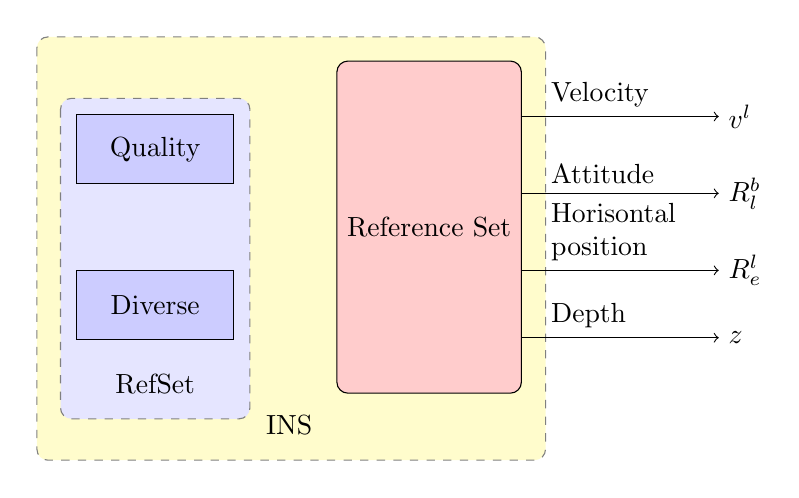
\begin{tikzpicture}
    \node (naveq) [naveqs] {Reference Set};
    % Note the use of \path instead of \node at ... below. 
    \path (naveq.140)+(-\blockdist,0) node (gyros) [sensor] {Quality};
    \path (naveq.-140)+(-\blockdist,0) node (accel) [sensor] {Diverse};
    
    %    \path [draw, ->] (gyros) -- node [above] {$\vc{\omega}_{ib}^b$} 
    %    (naveq.west |- gyros) ;
    % We could simply have written (gyros) .. (naveq.140). However, it's
    % best to avoid hard coding coordinates
    %      \path [draw, ->] (accel) -- node [above] {$\vc{f}^b$} 
    %      (naveq.west |- accel);
    \node (IMU) [below of=accel] {RefSet};
    \path (naveq.south west)+(-0.6,-0.4) node (INS) {INS};
    \draw [->] (naveq.50) -- node [ann] {Velocity } + (\edgedist,0) 
    node[right] {$\vc{v}^l$};
    \draw [->] (naveq.20) -- node [ann] {Attitude} + (\edgedist,0) 
    node[right] { $\mx{R}_l^b$};
    \draw [->] (naveq.-25) -- node [ann] {Horisontal position} + (\edgedist,0)
    node [right] {$\mx{R}_e^l$};
    \draw [->] (naveq.-50) -- node [ann] {Depth} + (\edgedist,0) 
    node[right] {$z$};
    
    % Now it's time to draw the colored IMU and INS rectangles.
    % To draw them behind the blocks we use pgf layers. This way we  
    % can use the above block coordinates to place the backgrounds   
    \begin{pgfonlayer}{background}
      % Compute a few helper coordinates
      \path (gyros.west |- naveq.north)+(-0.5,0.3) node (a) {};
      \path (INS.south -| naveq.east)+(+0.3,-0.2) node (b) {};
      \path[fill=yellow!20,rounded corners, draw=black!50, dashed]
      (a) rectangle (b);
      \path (gyros.north west)+(-0.2,0.2) node (a) {};
      \path (IMU.south -| gyros.east)+(+0.2,-0.2) node (b) {};
      \path[fill=blue!10,rounded corners, draw=black!50, dashed]
      (a) rectangle (b);
    \end{pgfonlayer}
  \end{tikzpicture}
  \caption{Scatter Search Update Method}
\end{figure}
\todo{Ajustar imagen si es que se va a dejar}
